
\input{../latex_main/main.tex}

%\newcommand{\a}[0]{\mathbf{a}}
%\newcommand{\y}[0]{\mathbf{y}}
\newcommand{\q}[0]{\mathbf{q}}
\newcommand{\Xspace}[0]{\mathcal{X}}
\newcommand{\inducer}{\mathcal{I}}

\title[AutoML: Overview]{Multi-criteria Optimization}
\subtitle{Practical Applications}
\author[Bernd Bischl]{\underline{Bernd Bischl} \and Frank Hutter \and Lars Kotthoff\newline \and Marius Lindauer \and Joaquin Vanschoren}
\institute{}
\date{}



% \AtBeginSection[] % Do nothing for \section*
% {
%   \begin{frame}{Outline}
%     \bigskip
%     \vfill
%     \tableofcontents[currentsection]
%   \end{frame}
% }

\begin{document}

	\maketitle

\begin{frame}[allowframebreaks]{Practical Applications in Machine Learning}

    \textbf{ROC Optimization}: Balance \emph{true positive} and \emph{false positive} rates
  \begin{itemize}
    \item Typically unbalanced classification tasks with unspecified costs.
    \item Could also use other ROC metrics, e.g., \emph{positive predicted value} or \emph{false discovery rate}.
  \end{itemize}

\textbf{Efficient Models}:
    Balance \emph{predictive performance} with \emph{prediction time}, \emph{energy consumption} and/or \emph{model size}.
  \begin{itemize}
    \item Time: Models in production need to predict fast.
    \item Size / Energy consumption: Models should be deployed on a mobile/edge device and not use much power.
    % \item Complexity: A model should be explainable.
  \end{itemize}
    
\textbf{Sparse Models}: Balance \emph{predictive performance} and \emph{number of used features}, either for cost effieciency, but often also for interpretability.

\textbf{Fair Models}:
  Balance \emph{predictive performance} and \emph{fairness}.
  \begin{itemize}
    \item Model has to be fair regarding subgroups in the data, e.g. gender.
    \item Many different approaches to quantify fairness exist.
  \end{itemize}


\end{frame}

\begin{frame}{ROC Optimization - Setup}

  Again, we want to train a \textit{spam detector} on the popular Spam dataset\footnote{\url{https://archive.ics.uci.edu/ml/datasets/spambase}}.

\begin{columns}
\begin{column}{0.5\textwidth}
\begin{itemize}
        \item Learning algorithm: SVM with RBF kernel.
        \item Hyperparameters to optimize: \\
        \begin{tabular}{rl}
        \texttt{cost} & $[2^{-15}, 2^{15}]$ \\
        $\gamma$ & $[2^{-15}, 2^{15}]$ \\
        Threshold $t$ & $[0,1]$ \\
        \end{tabular}
        \item Objective: \emph{minimize} false positive rate (FPR) and \emph{maximize} true positive rate (TPR), evaluated through 5-fold CV
\end{itemize}
\end{column}%
\begin{column}{0.5\textwidth}
\begin{itemize}
        \item Optimizer: Multi-criteria Bayesian optimization:
            \begin{itemize}
              \item ParEGO with $\rho = 0.05$, $s = 100000$.
              \item Acquisition function $\acq$: \emph{Confidence Bound} with $\alpha = 2$.
              \item Budget: $100$ evaluations
            \end{itemize}
        \item Tuning is conducted on a training holdout and all hyperparameter configurations on the estimated Pareto front are validated on an outer validation set.
\end{itemize}
\end{column}
\end{columns}
\vspace{0.5cm}
    {\footnotesize The threshold $t$ could be separately optimized post-hoc.}
\end{frame}

\begin{frame}{ROC Optimization - Result I}

\begin{columns}
\begin{column}{0.45\textwidth}
  We notice:
  \begin{itemize}
    \item Compared to \emph{random search}: Many \emph{ParEGO} evaluations are on the Pareto front.
    \item The Pareto front of \emph{ParEGO} dominates most points from the \emph{random search}.
    \item The dominated hypervolume to the reference point $(0,1)$ is:
    \begin{tabular}{rl}
    \emph{ParEGO:} & 0.965\\
    \emph{random search:} & 0.959\\
    \end{tabular}
  \end{itemize}
  %Note: The Pareto front does not reflect the stochastic characteristic of our objective.
\end{column}%
\begin{column}{0.5\textwidth}
  \begin{figure}
  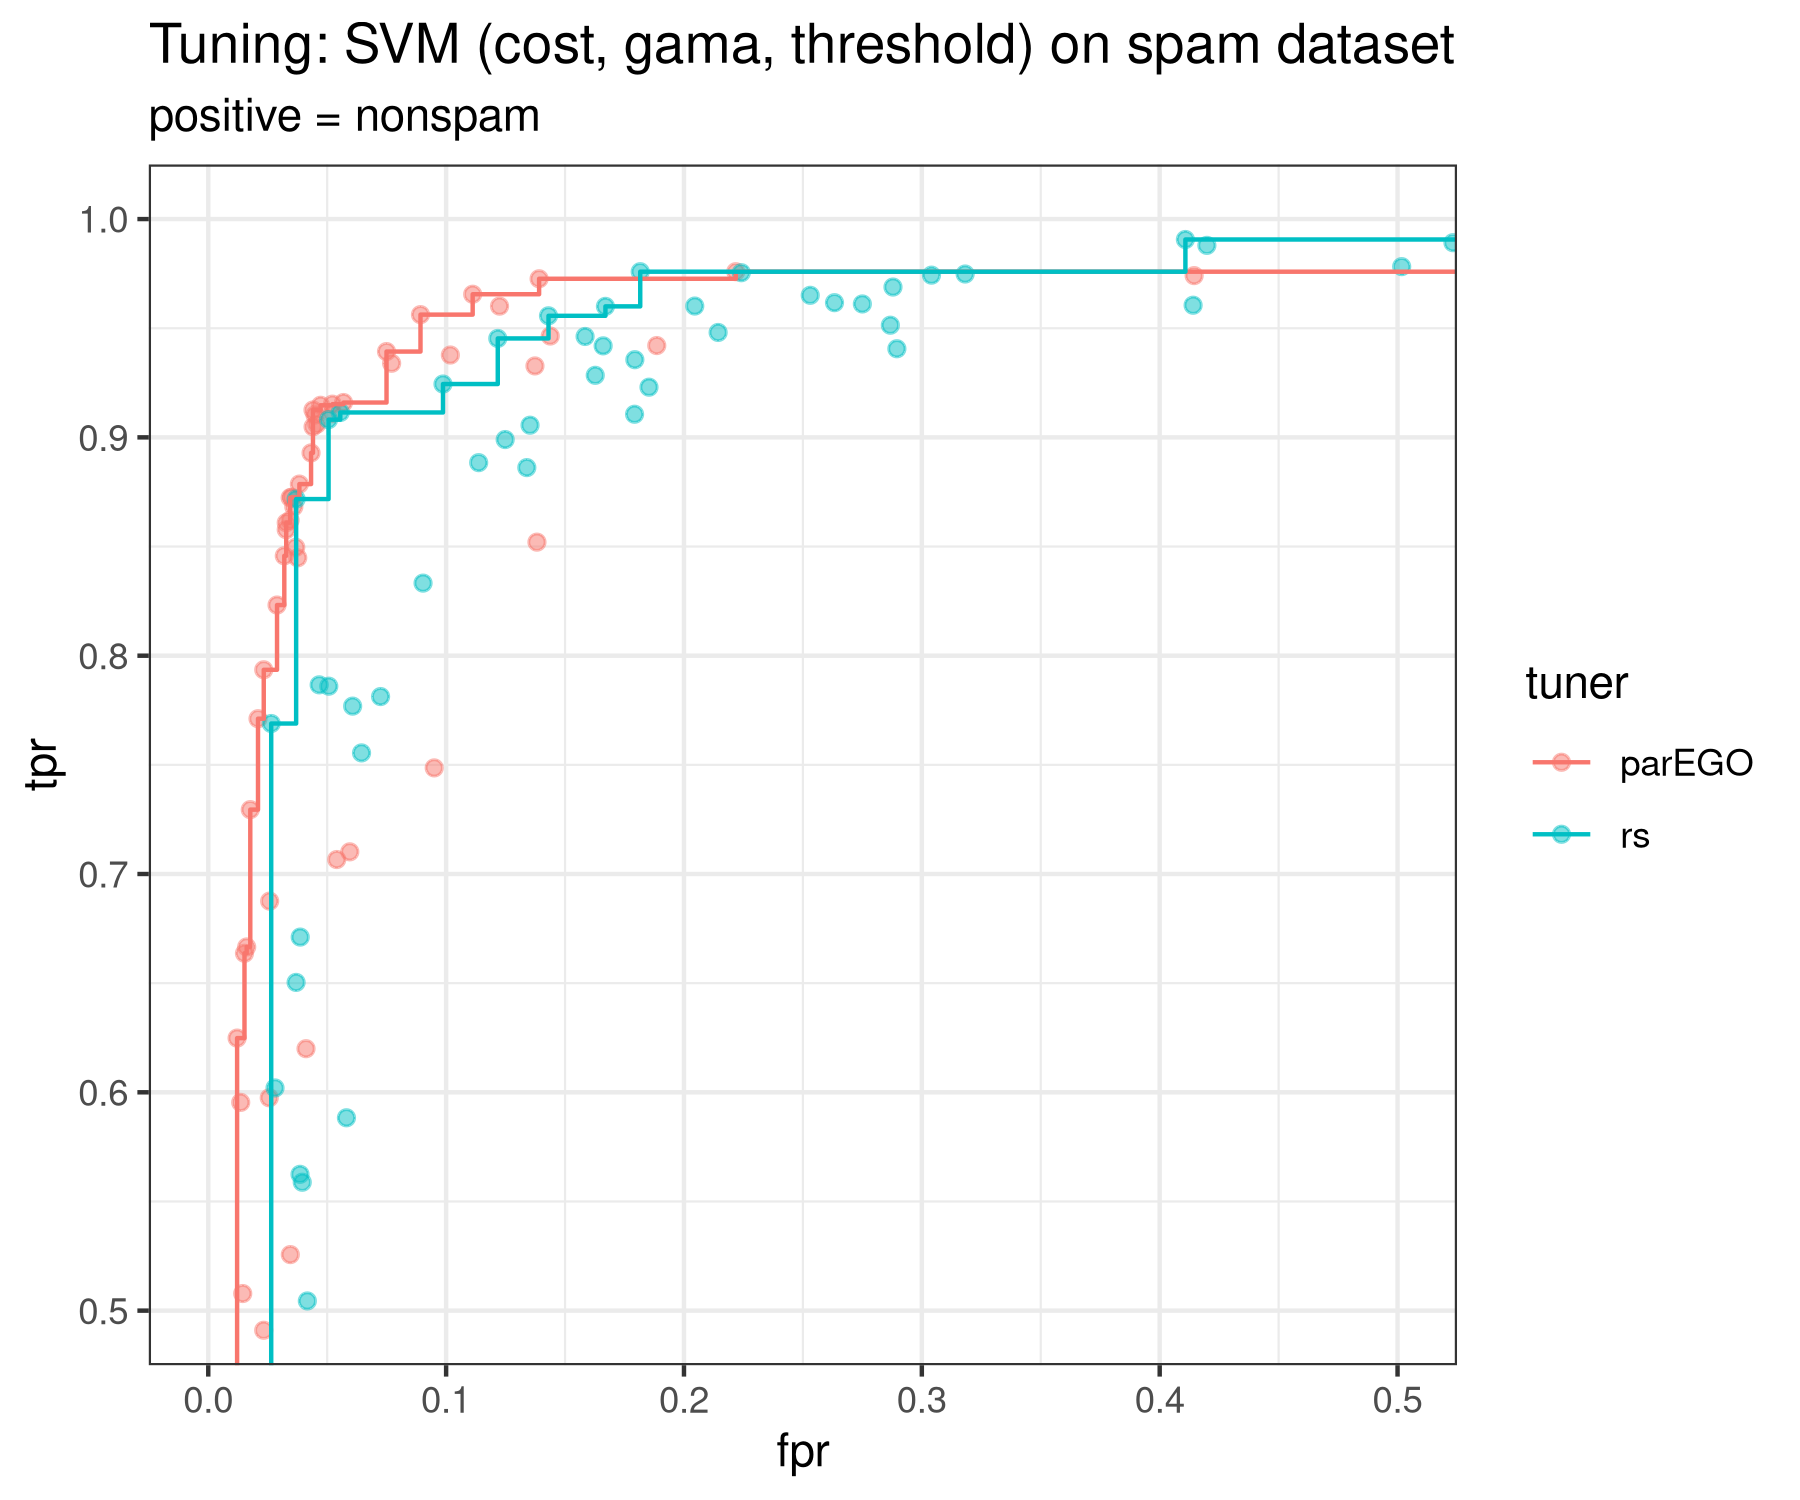
\includegraphics[width=\textwidth]{images/example_parego_spam.png}
  \end{figure}
\end{column}
\end{columns}

\end{frame}

\begin{frame}{ROC Optimization - Result II}

\begin{columns}
\begin{column}{0.45\textwidth}
  We validate the configurations on the estimated Pareto front on a holdout:
  \begin{itemize}
    \item<1-> The performance on the validation set varies slightly.
    \item<1-> The TPR got slightly better but the FPR got slightly worse.
    \item<1-> On the validation set, some configurations get dominated by others.
    \item<2> The dominated hypervolume of the validation set is:
    \begin{tabular}{rl}
    \emph{ParEGO:} & 0.960\\
    \emph{random search:} & 0.961\\
    \end{tabular}
  \end{itemize}
\end{column}%
\begin{column}{0.5\textwidth}
  \begin{figure}
  \includegraphics<1>[width=\textwidth]{images/example_parego_spam_outer.png}
  \includegraphics<2>[width=\textwidth]{images/example_parego_spam_outer_pareto.png}
  \end{figure}
\end{column}
\end{columns}

\end{frame}

\begin{frame}{Efficient Models - Overview}

\begin{itemize}
  \item "Efficiency" can be:
  \begin{itemize}
    \item Memory consumption of the model
    \item Training or prediction time
    \item Number of features needed
    \item Energy consumption for prediction
    \item \ldots
  \end{itemize}
  \item Some hyperparameters have a strong impact on the efficiency of a model, e.g.,
  \begin{itemize}
    \item Number of trees in \emph{random forests} or \emph{gradient tree boosting},
    \item Number, size and type of layers in \emph{neural networks},
    \item L1 regularization penalties,
    \item ...
  \end{itemize}
  \item Other hyperparameters might have no influence on efficiency.
  \item Typical scenario: Optimize jointly over multiple algorithms of varying efficiency.
\end{itemize}

\end{frame}

\begin{frame}{Efficient Models - Example: Feature Selection I}

Goal of \emph{feature selection}: Identify an informative feature subset with only a small drop in predictive performance compared to all features.

    \vspace{0.5cm}
Find optimal hyperparameter setting $\conf$ and minimal feature subset $s$
\[
\min_{\conf \in \pcs, s \in \{0,1\}^p}\left( \widehat{GE}\left(\inducer(\dataset, \conf, s)\right), \frac{1}{p}\sum_{i=1}^p s_i \right)
\]
\begin{itemize}
  \item Problem: Feature selection and hyperparameter tuning are usually two separate steps.
  \item Solution: Identify an informative subset of features and a good hyperparameter configuration \textbf{simultaneously}.

\end{itemize}
\begin{figure}
  \centering
  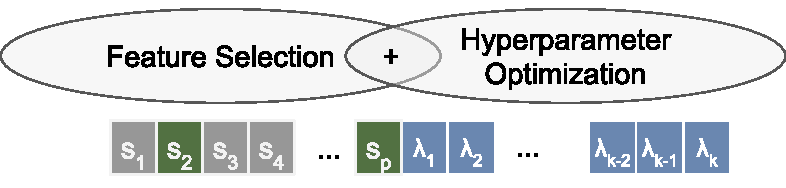
\includegraphics[width = 0.5\linewidth]{images/mosmafs_presentation_p14.pdf}
\end{figure}

\end{frame}

\begin{frame}{Efficient Models - Example: Feature Selection II}
Idea: \emph{Multi-Objective Hyperparameter Tuning and Feature Selection using Filter Ensembles}~\lit{\href{https://arxiv.org/pdf/1912.12912.pdf}{Binder et al. 2020}}:


  \begin{itemize}
    \item Pre-calculate multiple ranked \emph{feature filter values} .

    \begin{figure}
      \centering
      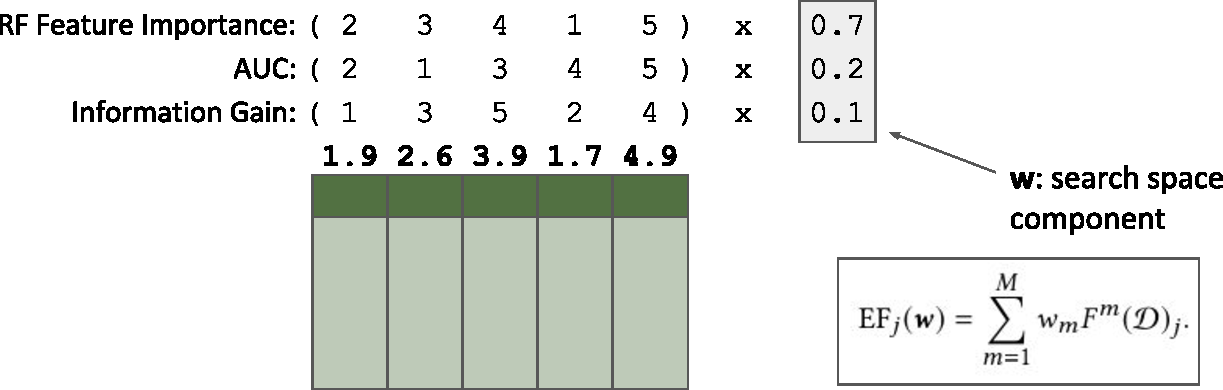
\includegraphics[width = 0.7\linewidth]{images/mosmafs_presentation_p39.pdf}
    \end{figure}

    \item New joint hyperparameter vector: $\conf = (\tilde{\conf}, w_1, \ldots, w_p ,\tau )$
    \begin{itemize}
      \item Hyperparameters of learner: $\tilde{\conf}$
      \item Weight of each \emph{feature filter value} vector: $(w_1, \ldots, w_p)$
      \item Fraction of features to keep $\tau$
    \end{itemize}

  \end{itemize}

\end{frame}

\begin{frame}{Efficient Models - Example: Feature Selection III}
    Combined feature selection and hyperparameter optimization on \texttt{Sonar} dataset\footnote{Only the tuning error is shown here}.
\begin{columns}
\begin{column}{0.65\textwidth}
  \begin{itemize}
    \item Learning algorithm: SVM with RBF kernel.
    \item Hyperparameters to optimize: \\
    \begin{tabular}{rl}
    \texttt{cost} & $[2^{-10}, 2^{10}]$ \\
    $\gamma$ & $[2^{-10}, 2^{10}]$ \\
    $(w_1, \ldots, w_p)$ & $[0,1]^p$ \\
    $\tau$ & $[0,1]^p$ \\
    \end{tabular}
    \item Objective: minimize \emph{misclassification} and \emph{fraction of features selected}
    \item Optimizer: \emph{ParEGO} with \emph{random forest} surrogate, LCB acquisition function, 15 batch proposals, budget: 2000 evaluations
  \end{itemize}
\end{column}%
\begin{column}{0.35\textwidth}

  \begin{figure}
    \centering
    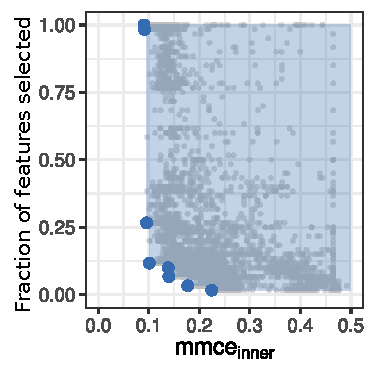
\includegraphics[width=\linewidth]{images/mosmafs_sonar_eval_domHV.pdf}
    %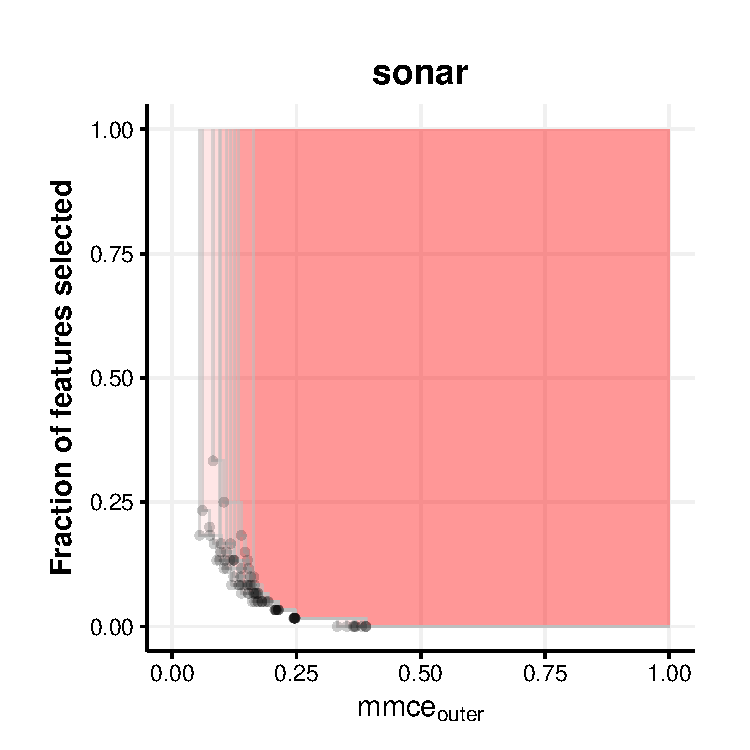
\includegraphics[width=\linewidth]{images/mosmafs_sonar_front.pdf}
  \end{figure}

\end{column}
\end{columns}
\end{frame}

\begin{frame}{Efficient Models - Example: FLOPS}

    Goal: Optimize prediction accuracy and number of floating point operations (FLOPs)~\\ \lit{\href{https://arxiv.org/pdf/1904.09035.pdf}{Wang et al. 2019}}.

    \vspace{0.5cm}

    Data: Image Classification on CIFAR-10.

    \vspace{0.5cm}

    Learner: \emph{DenseNet} - Densely Connected Convolutional Network~\lit{\href{https://arxiv.org/pdf/1608.06993.pdf}{Huang et al. 2018}}.

    \begin{itemize}
        \item Composed out of $4$ \emph{dense blocks}.
        \item A dense block consists of multiple convolutional layers where the inputs for each layer are all feature maps of all preceding layers in the block.
        \item Dense blocks are connected via convolutional and max pooling layer.
    \end{itemize}

    \vspace{0.5cm}

    Training: $300$ Epochs with a batch size of $128$ and initial learning rate of $0.1$.

\end{frame}

\begin{frame}{Efficient Models - Example: FLOPS}
\begin{columns}
  \begin{column}{0.65\textwidth}
    \begin{itemize}
      \item Objective: \emph{accuracy} vs.\ \emph{FLOPS} (floating point operations, per observation)
      \item Search Space:\\
        \begin{tabular}{rl}
            \texttt{growth rate} ($k$) & $[8,32]$ \\ %growth rate: k_l = k_0 + k (l-1), how much information is added in each layer
          \texttt{layers in first block} & $[4, 6]$ \\
          \texttt{layers in second block} & $[4, 12] $ \\
          \texttt{layers in third block} & $[4, 24] $ \\
          \texttt{layers in fourth block} & $[4, 16] $ \\
        \end{tabular}
      \item Tuner: \emph{Particle Swarm Optimization} with a population size of $20$ and $400$ evaluations.
    \end{itemize}
  \end{column}%
  \begin{column}{0.35\textwidth}
    \begin{figure}
    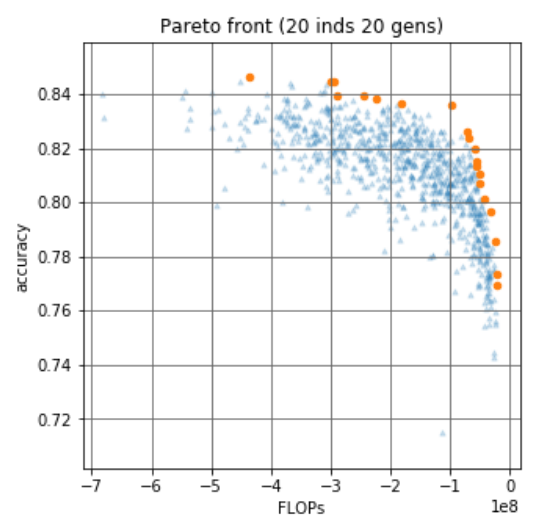
\includegraphics[width=\textwidth]{images/Wang_et_al_2019_Evolving_Deep_Neural_Networks_fig7_1.png}
    \end{figure}
  \end{column}
  \end{columns}

    {\footnotesize The \texttt{growth rate} is the number of output feature maps in each layer of a block}

\end{frame}

\begin{frame}{Fair Models - The \texttt{Adult} dataset}
\begin{columns}
\begin{column}{0.4\textwidth}
Dataset: \texttt{Adult}
\begin{itemize}
  \footnotesize
  \item  Source: US Census database, 1994, \url{https://www.openml.org/d/1590}.
  \item 48842 observations
  \item Target: binary, income above 50k
  \item 14 features: \texttt{age, education, hours.per.week, marital.status, native.country, occupation, race, relationship, sex, \ldots}
\end{itemize}
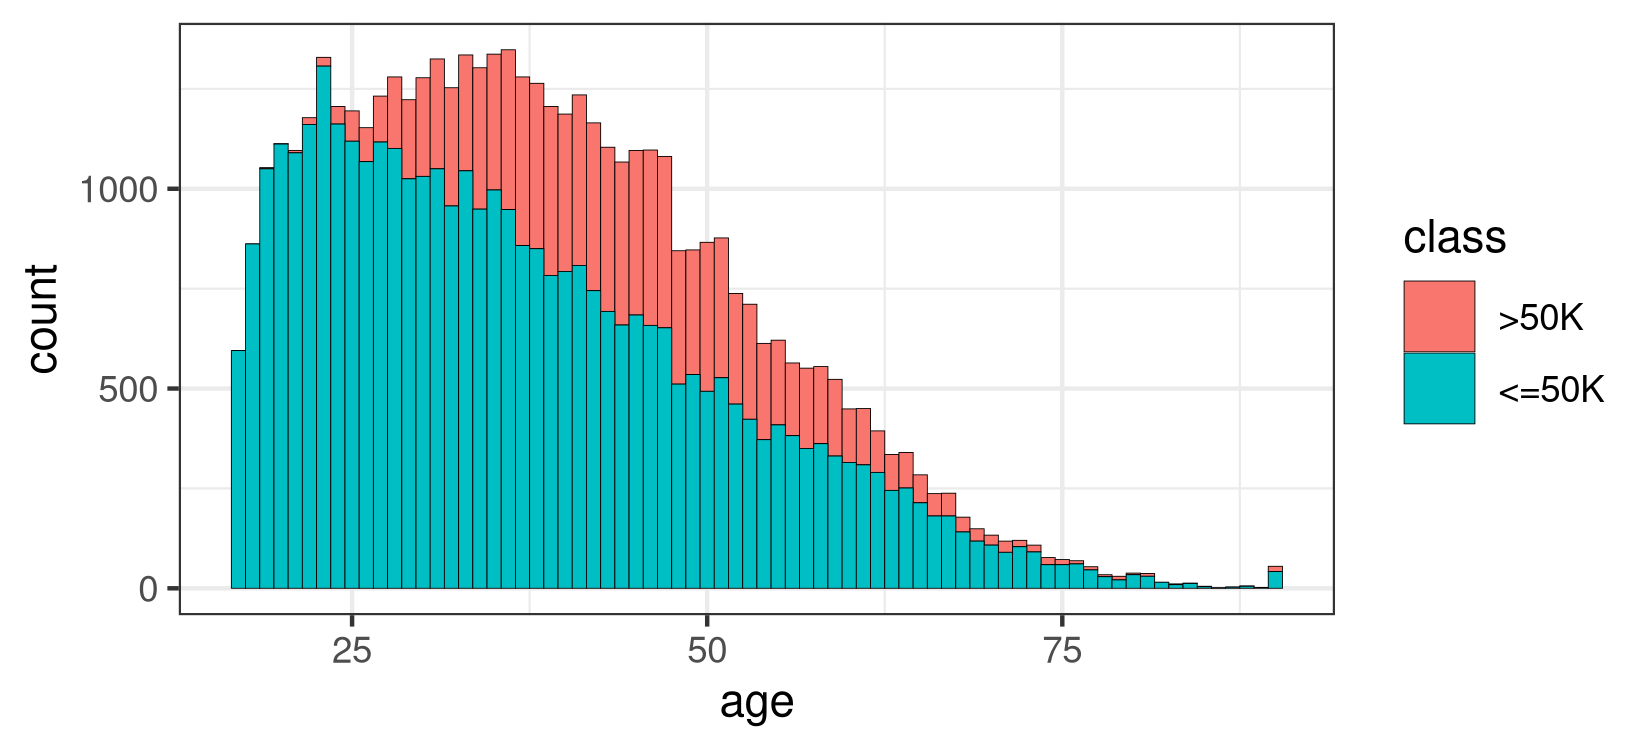
\includegraphics[scale = 0.45]{images/dataset_adult_age_sex.png}
\end{column}%
\begin{column}{0.6\textwidth}

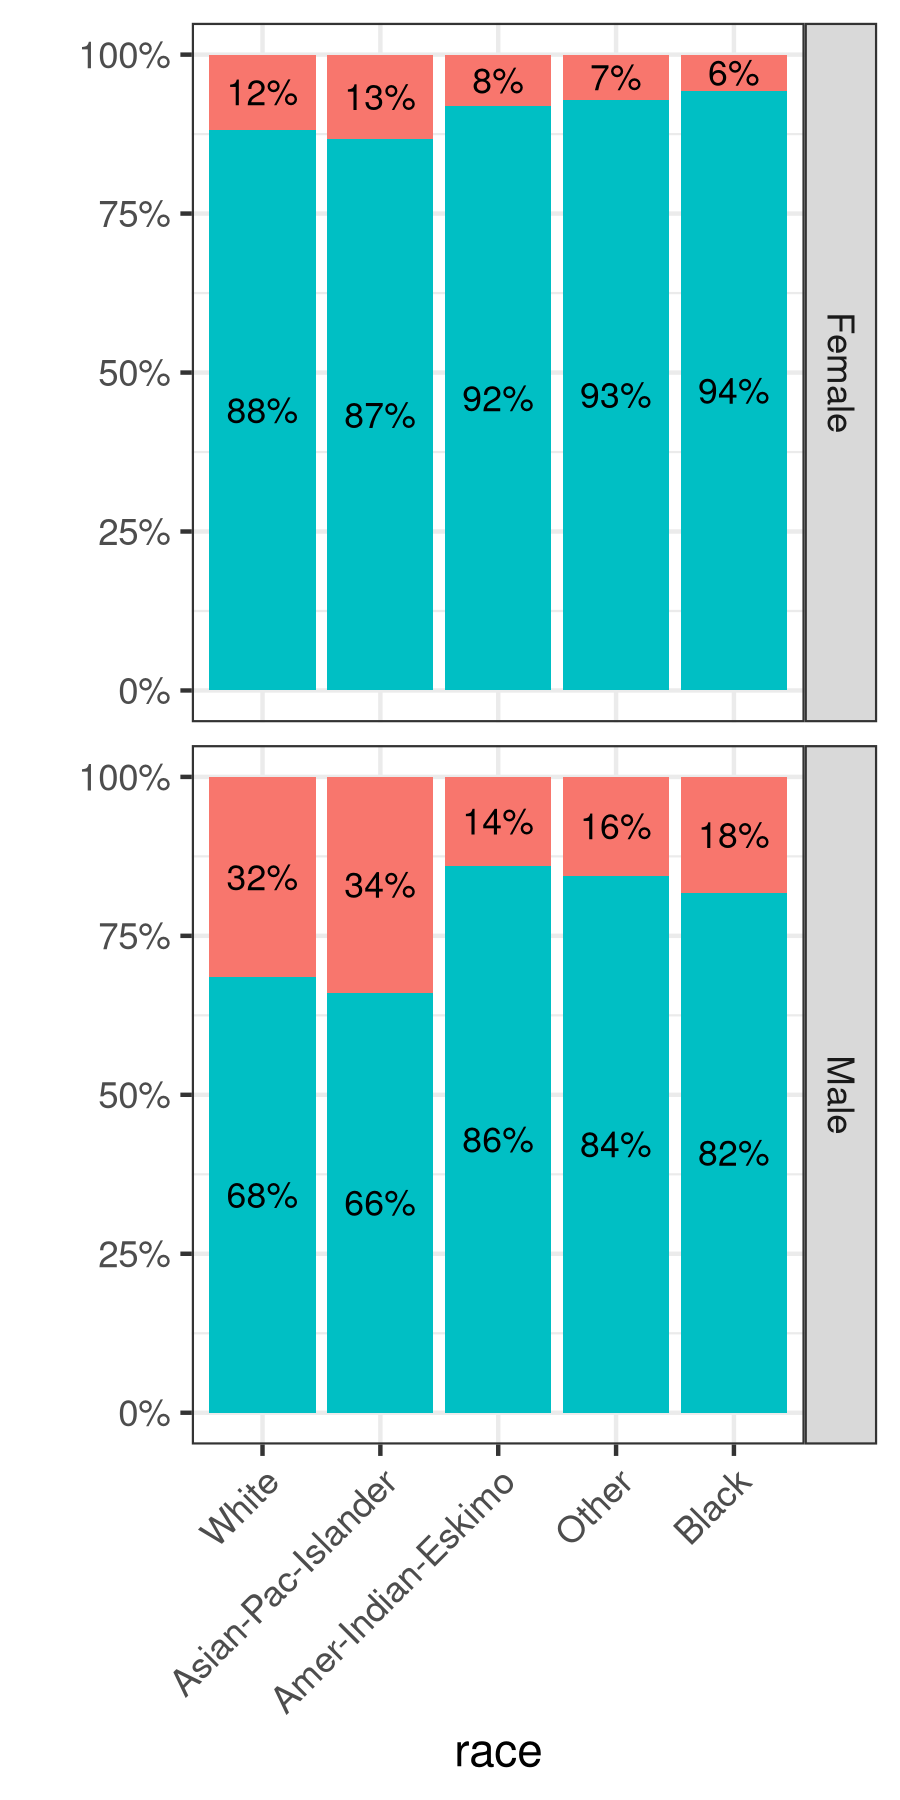
\includegraphics[scale = 0.45]{images/dataset_adult_race.png}%
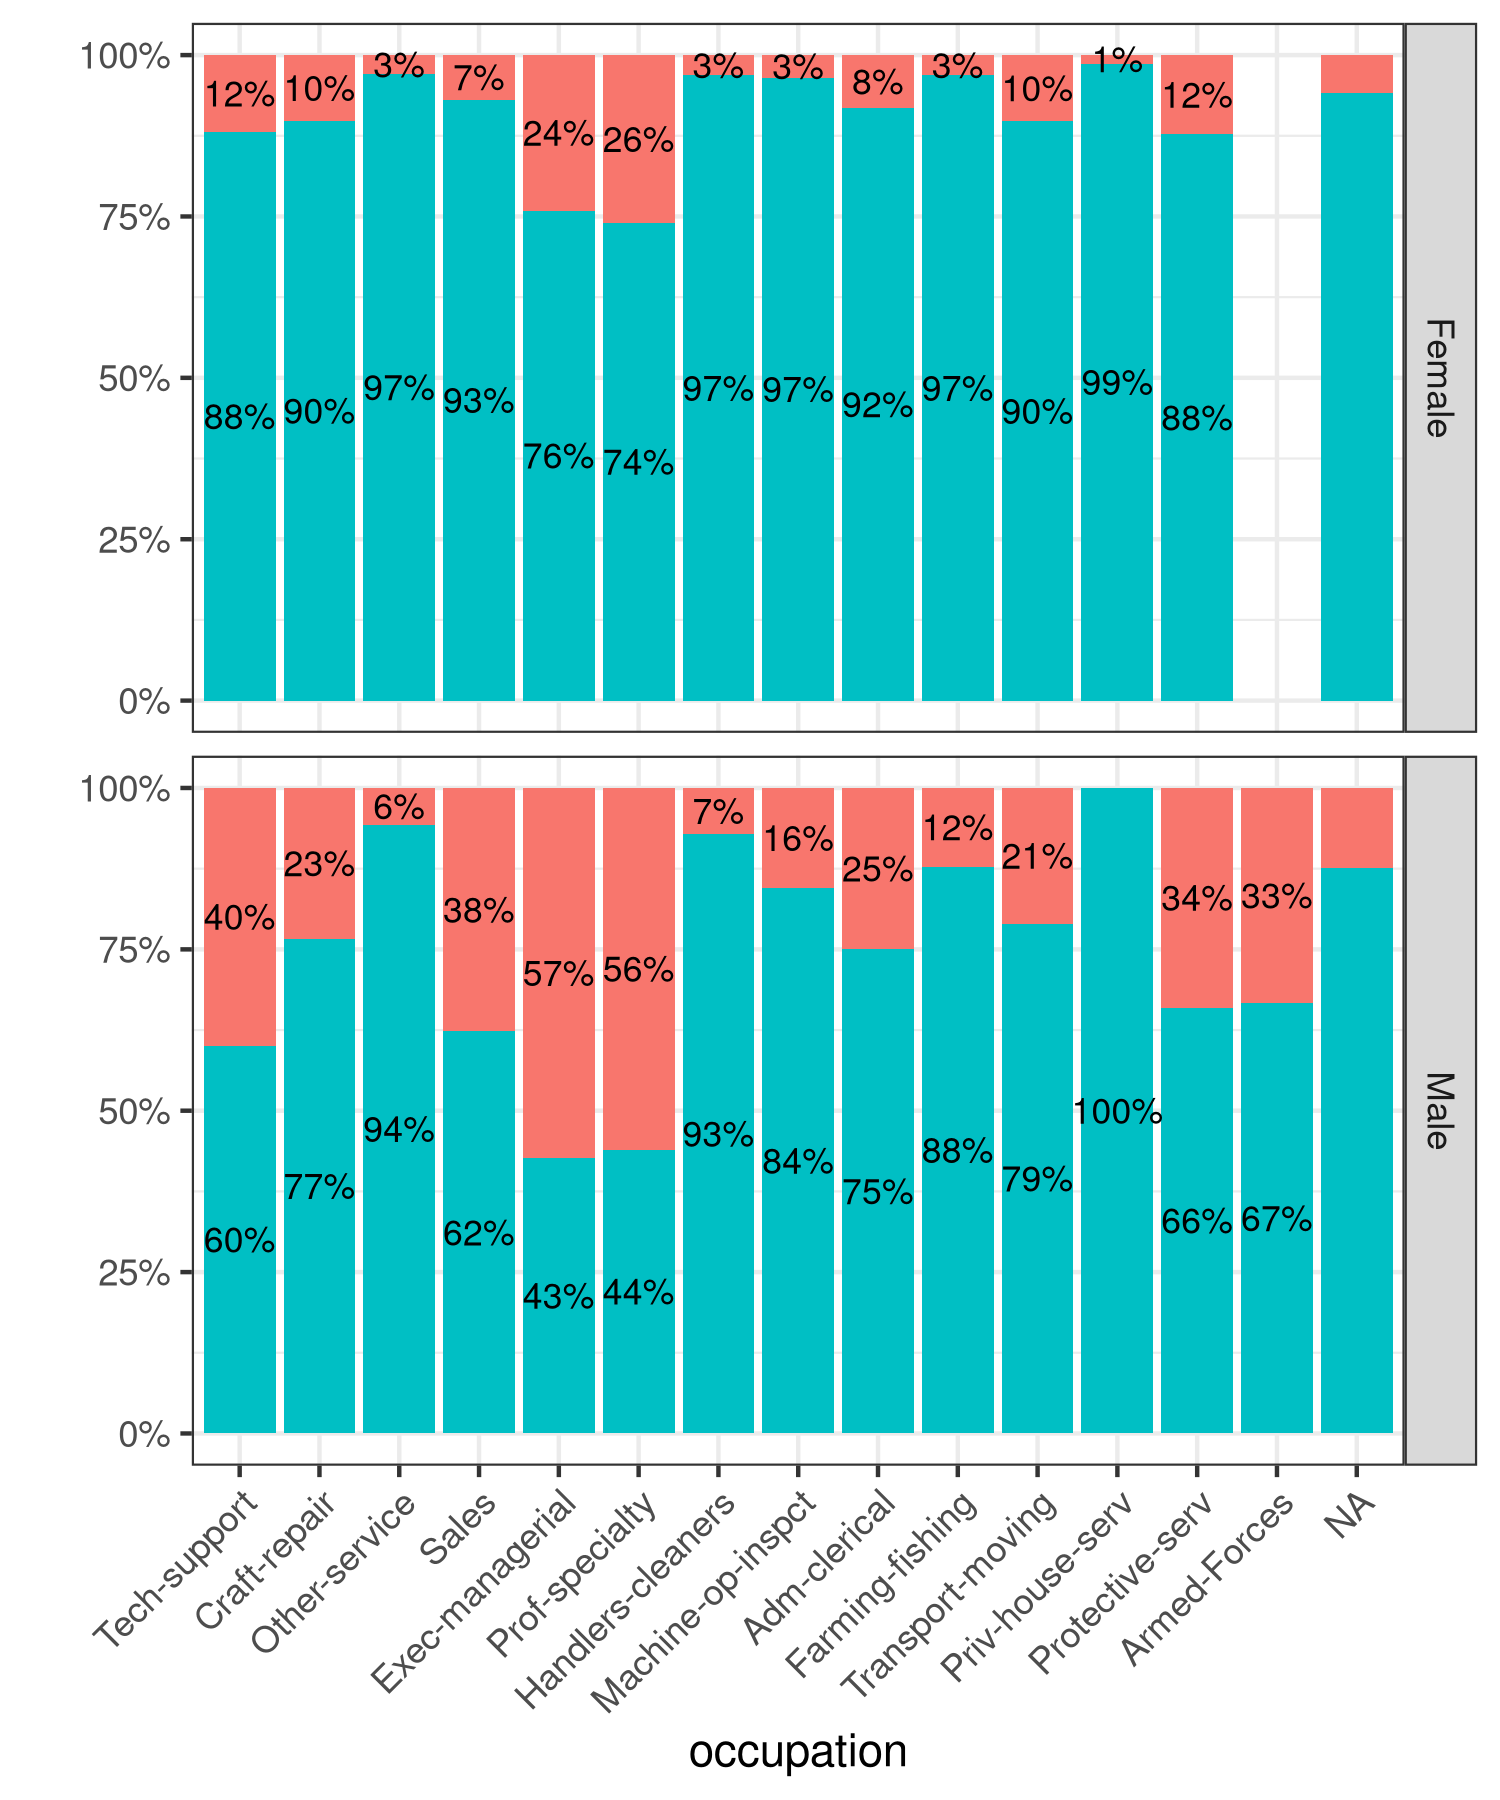
\includegraphics[scale = 0.45]{images/dataset_adult_education.png}
\end{column}
\end{columns}


\end{frame}

\begin{frame}[allowframebreaks]{Fair Models - Setup}
  A fair model for income prediction on binarized target.
%\begin{columns}
%\begin{column}{0.5\textwidth}
\begin{itemize}
  \item Learner: \emph{eXtreme Gradient Boosting}
  \item Hyperparameters to optimize: \\
  \begin{tabular}{rl}
    \texttt{eta} & $[0.01,0.2]$ \\
    \texttt{gamma} & $[2^{-7},2^6]$ \\
    \texttt{max\_depth} & $\{2, \ldots, 20\}$ \\
    \texttt{colsample\_bytree} & $[0.5,1]$ \\
    \texttt{colsample\_bylevel} & $[0.5,1]$ \\
    \texttt{lambda} & $[2^{-10},2^{10}]$ \\
    \texttt{alpha} & $[2^{-10},2^{10}]$ \\
    \texttt{subsample} & $[0.5,1]$ \\
  \end{tabular}
  \item Objective: minimize \emph{misclassification error} and \emph{unfairness}
%\end{itemize}
%\end{column}%
%\begin{column}{0.5\textwidth}
%\begin{itemize}
  \item Careful: Usually this data would be used to model the relation between person characteristics and income, then to \textbf{discuss and study} by careful inference - to \textbf{figure out if} something like e.g. a "gender pay gap" exists.
  \item Here, in our toy example we \textbf{pretend} now that we would like to create a automatic "assignment algorithm" for salary - maybe not totally unrealistic nowadays? In \textbf{such} a scenario, biasing the prediction by \textbf{incorporating fairness} might be of interest.
  % \item Question: Is the rate of classified as \emph{high income} equal amongst both subgroups given the prevalence in each subgroup?
  \item Here, a simplified proxy for fairness is defined as the absolute difference in F1-Scores between female ($f$) and male ($m$) population (low is good):
  \[
  \loss_{\text{fair}} := |\loss_{\text{F1}}(y_f,\fh(\x_f)) - \loss_{\text{F1}}(y_m,\fh(\x_m))|
  \]
\end{itemize}
\vspace{1em}
%\end{column}
%\end{columns}

\end{frame}

\begin{frame}{Fair Models - Results}

  \begin{figure}
    \centering
    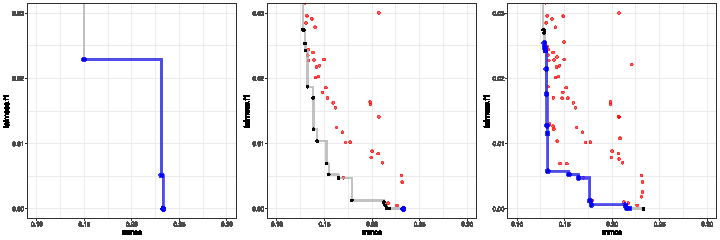
\includegraphics[scale=1.0]{images/Pfisterer_et_al_2019_Multi_Objective_fig4.pdf}
    \caption{Pareto fronts after 20, 70 and 120 tuning iterations.}
  \end{figure}

\begin{itemize}
  \item Optimizer: ParEGO with random forest surrogate and restricted range of projections to $[0.1, 0.9]$ (No interest in very unfair or bad configurations).
  \item Here, the hyperparameters actually have an effect on the defined \emph{fairness measure}.
  \item However, this is often not the case or not enough to ensure a fair model.
\end{itemize}
  

\end{frame}



\end{document}
